\chapter{Electrones en un potencial periódico. Teoría de bandas.} \label{Ch:07}

Para mejorar algunas de las predicciones del modelo del gas de electrones libres se introduce ahora la interacción de los electrones con la red cristalina a través de un potencial periódico. Se sigue despreciando, sin embargo, la posible interacción de los electrones entre sí.

\section{Teorema de Bloch}

Se estudia el comportamiento de un electtón en un potencial con la propiedad $U(\rn)= U(\rn+\Rn)$ siendo $\Rn$ un vector de red. El hecho de que este potencial sea periódico permite establecer la forma general que debe  tener la función de onda. La ecuación de Schrödinger para un electrón es

\begin{equation}  
    - \frac{\hbar^2}{2m} \nabla^2 \Psi (\rn) + U(\rn) \Psi (\rn) = \varepsilon \Psi (\rn) \label{Ec:07-01-01}
\end{equation}
Supongamos el nivel $\varepsilon$ no degenerado (aunque el resultado final no dependa de esta circunstancia). El hecho de que $\Psi (\rn+ \Rn)$ sea también solución de (\ref{Ec:07-01-01}) exige a la función ser igual que $\Psi(\rn)$ salvo por una constante (que puede ser compleja) $\Psi (\Rn+\rn)=C(\Rn) \Psi (\rn)$. Como $\Psi(\rn)$ y $\Psi (\rn + \Rn)$ deben estar normalizadas, se tiene que $|C|^2 = 1 \rightarrow C(\Rn)=e^{i \phi(\Rn)}$. Para dos traslaciones sucesivas $C(\Rn) C(\Rn') = C(\Rn+\Rn')$, que se verifica si $\phi(\Rn)=\kn \cdot \Rn$ donde $\kn$ es un vector constante. En resumen, para cualquier nivel $\varepsilon$ las autofunciones verifican 

\begin{eqnarray}
    \Psi (\rn + \Rn) = e^{i\kn \cdot \Rn} \Psi (\rn) \label{Ec:07-01-02}
\end{eqnarray}
Podemos etiquetar los autoestados por un vector $\kn$ que denominaremos como \textbf{vector de onda}, y entonces $\varepsilon=\varepsilon(\kn)$. Una forma equivalente de (\ref{Ec:07-01-02}) es-nodecimaldot

\begin{eqnarray}
    \Psi (\rn) = u_{\kn} (\rn) e^{i \kn \cdot \rn} \label{Ec:07-01-03}
\end{eqnarray}
donde $u_{\kn} (\rn + \Rn) = u_{\kn} (\rn)$. Este resultado se conoce como \textit{teorema de Bloch}. La solución general (función de onda Bloch) es una onda plana modulada en amplitud. Algunas de las consecuencais que se derivan de (\ref{Ec:07-01-03}) son:

\begin{itemize}
    \item $\kn$ está definido en un vector $\Gn$ perteneciente a la red recíproca, pues si $\kn$ verifica (\ref{Ec:07-01-01}) también lo hace $\kn + \Gn$, y por tanto también $\varepsilon(\kn)=\varepsilon (\kn + \Gn)$. 
    \item La combinación $\hbar \kn$, denominada cuasiimpulso no es el impulso del electrón, pues $i\hbar \nabla \Psi_{\kn} \neq \hbar \kn \Psi_{\kn}$, lo que es consistente pues el impulso no debe ser una constante de movimiento en un potencial periódico.
    \item Por ser hamiltoniano hermítico se puede probar que $\varepsilon(\kn)=\varepsilon(-\kn)$.
    \item Se verifica $|\Psi (\rn) |^2 = |\Psi (\rn + \Rn)|^2$, como debe ser en una estructura periódica.
    \item Al imponer las condiciones de contorno periódicas, los valores de $\kn$ distintos (en una celda primitiva de la red recíproca) son los mismos ya vistos en el Capítulo anterior, esto es, igual al número $N$ de celdas primitvas de la red directa.
\end{itemize}

\section{Aproximación de red vacía}


Se trata de ver los cambios que introduce un potencial periódico (``red'') tan débil que no afecte apreciablemente al espectro de energías del electrón libre:

\begin{equation}
    \varepsilon (\kn) \approx \varepsilon_0 (\kn) \equiv \frac{\hbar^2 k^2}{2m}
\end{equation}
de ahí lo de ``vacía''. En la discusión supondremos 1D para simplificar. Como $\varepsilon(k) = \varepsilon(k+G)$, la relación de dispersión sería la representada en la figura \ref{Fig:07-01} (arriba). Esta reprsentación se denomina \textit{esquema en zona periódica}. Obsérvese que si contamos las porciones de las distintas parábolas que entran en la PZB ya se contabilizan todas las soluciones posibles ($\varepsilon(k)$) de la partícula libre. Se tiene así el llamado \textit{esquema en zona reducida}, representado en la figura \ref{Fig:07-01} (abajo izquierda), donde se ve claro la existencia de mcuhas soluciones para cada valor de $k$. En concreto, todas las energías se pueden representar por 

\begin{equation}
    \varepsilon_0 (k_{\PZB}) = \frac{\hbar^2 (k_{\PZB}-G)^2}{2m}
\end{equation}
para los distintos $G$ de la red recíproca. Los valores posibles de energía se clasfiican en \textit{bandas de energías}. Así como en este caso todas las energías son posibles, veremos que la presencia de un potencial periódico no despreciable puede introducir intervalos prohibidos de energía entre las diferentes bandas (de ahí toma sentido el concepto de \textit{banda de energía}). Una última reprsentación de la relación de dispersión es el llamado \textit{esquema en zona extendida} en el que cada banda se representa en una zona de Birllouin distitna (figura \ref{Fig:07-01} abajo derecha) (es necsario recordar que la zona $n$-ésima de Brillouin se define como la región del esapcio $k$ a la que se puede acceder desde el origen atravesando $n-1$ planos de Bragg). Aquí nos e aplica $\varepsilon(k) = \varepsilon(k+G)$ pues ya se ha eliminado la redundancia de información.

\begin{figure}[h!] \centering
    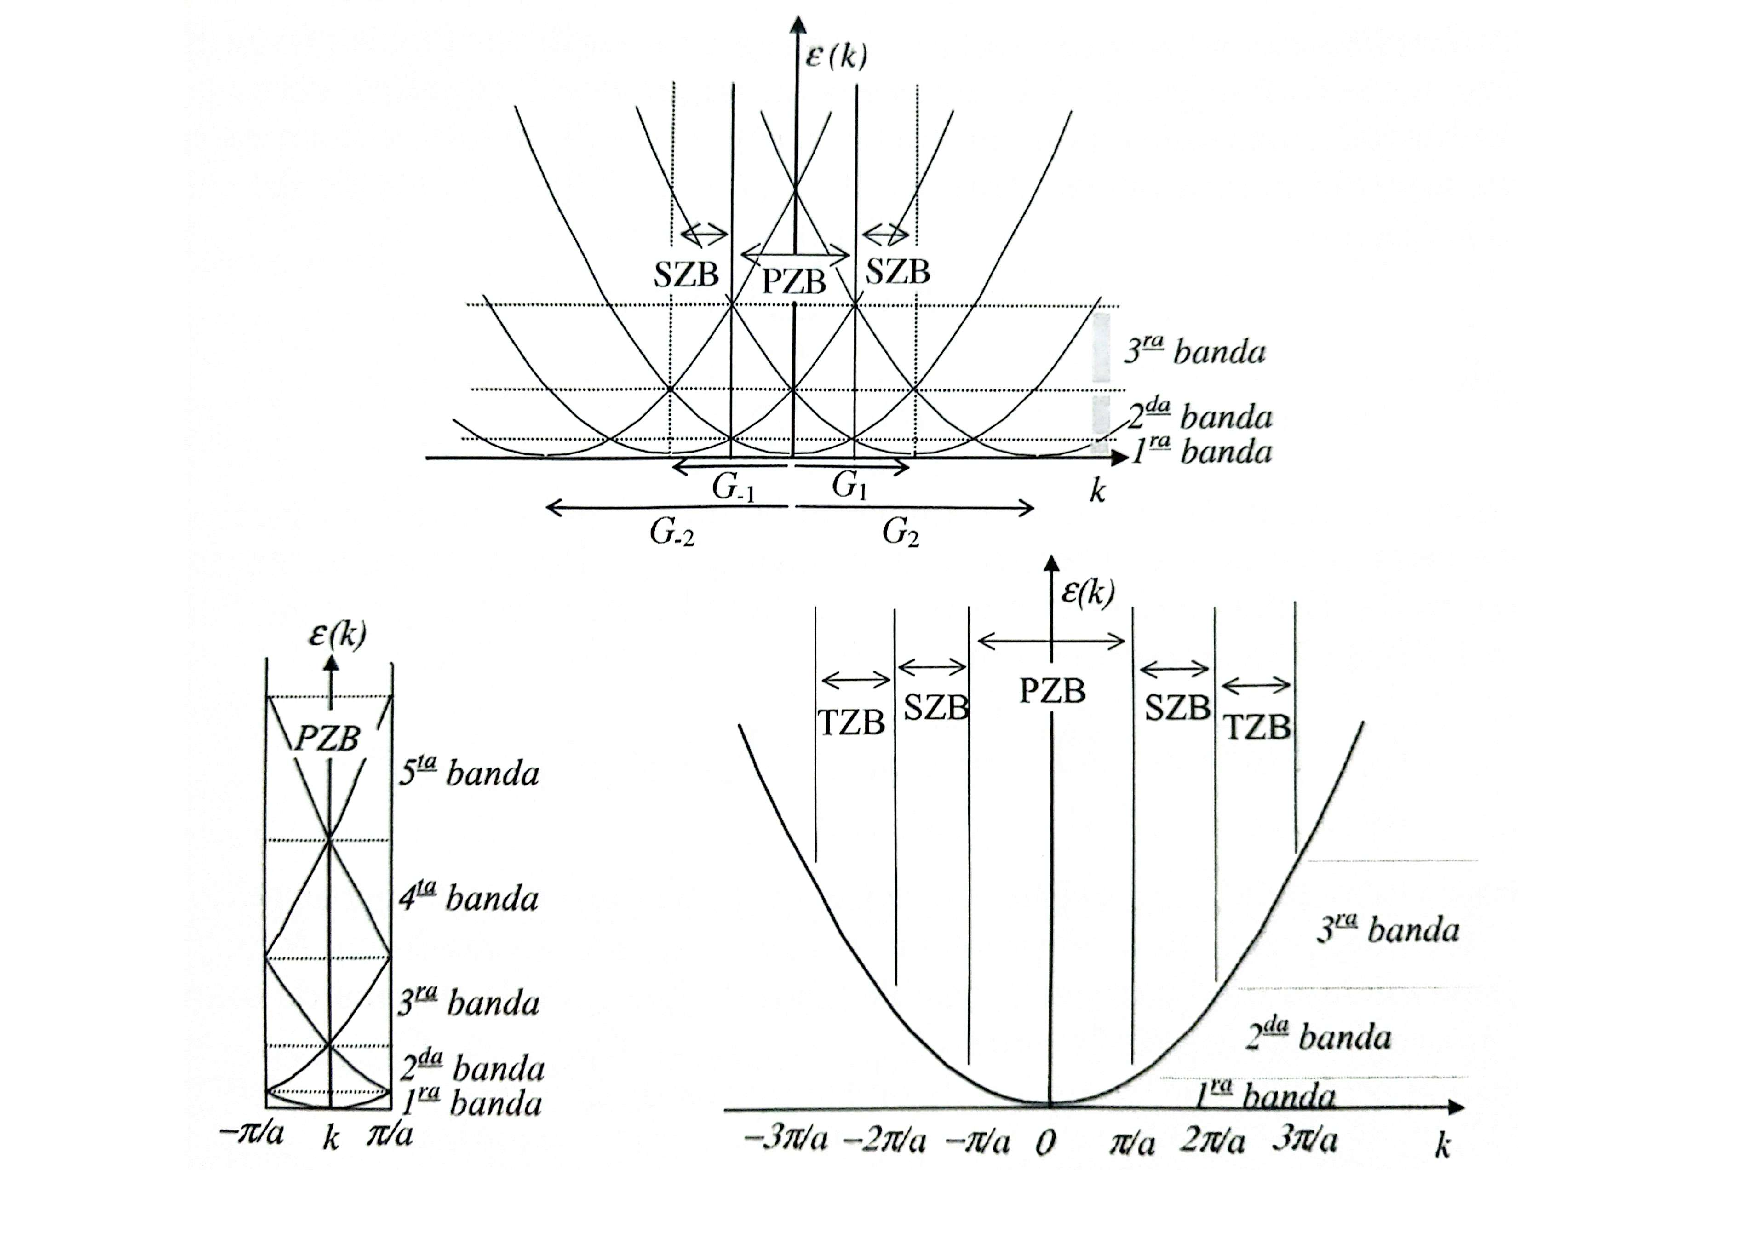
\includegraphics[scale=0.5]{Cuerpo/Ch_07/Fotos libro 1.pdf}
    \caption{Arriba: Esquema en zona periódica. Abajo: Esquemas en zona reducida (izquierda) y en zona extendida (derecha).}
    \label{Fig:07-01}
\end{figure}    

\section{Ecuación de onda del electrón en un potencial periódico}

La función de onda se puede expresar de manera general por la suma de Fourier:

\begin{equation}
    \Psi (\rn) = \sum_{\kn} C_{\kn} e^{-i\kn \cdot \rn} \label{Ec:07-03-01}
\end{equation}
para todos los $\kn$ que cumplen las condiciones de contorno. Nuestro objetivo es determinar los coeficientes de $C$ en (\ref{Ec:07-03-01}) bajo distintas aproximaciones para $U(\rn)$. Al ser periódico el potencial $U(\rn)$, se podrá escribir como

\begin{eqnarray}
    U(\rn) = \sum_{\Gn} U_{\Gn} U_{\Gn} e^{i \Gn \cdot \rn}
\end{eqnarray}
donde 

\begin{eqnarray}
    U_{\Gn} = \frac{1}{V_{\text{celda}}} \int_{\text{celda}} e^{-i \Gn \cdot \rn} U(\rn) \D \rn \label{Ec:07-03-03}
\end{eqnarray}
Por simplificar, tomaremos el origen de la energía de modo que la energía media sea nula, es decir, $U_{\Gn=0}=0$, y escogemos el origen de coordenadas de modo que el potencial tenga simetría de inversión $U(\rn)=U(-\rn)$, lo que es siempre posible para una red monoatómica. Tras sustituir (\ref{Ec:07-03-01}) y (\ref{Ec:07-03-03}) en la ecuación de Schrödinger (\ref{Ec:07-01-01}), resulta:

\begin{eqnarray}
    \ccorchetes{\varepsilon_0 (\kn) - \varepsilon} C_\kn + \sum_{\Gn} U_\Gn C_{\kn-\Gn}=0 \label{Ec:07-03-04}
\end{eqnarray}
con 
\begin{eqnarray}
\varepsilon (\kn)\equiv \frac{\hbar^2 k^2}{2m}  \label{Ec:07-03-05}
\end{eqnarray}
para cada valor de $\kn$ compatible con las condiciones de contorno. Si introducimos $\kn_{\PZB}=\kn+\Gn$ donde $\Gn$ es cierto vecetor de la red recíproca tal que $\kn_{\PZB}$ pertenece a la PZB, la ecuación (\ref{Ec:07-03-04}) se reescribe como

\begin{eqnarray}
\ccorchetes{\varepsilon_0 \parentesis{\kn_{\PZB} - \Gn} - \varepsilon} C_{\kn_{\PZB}-\Gn}  + \sum_{\Gn'} U_{\Gn'-\Gn} C_{\kn_{\PZB}-\Gn'} = 0  \label{Ec:07-03-06}
\end{eqnarray}
Ahora, para cada $\kn_{\PZB}$ existe una ecuación (\ref{Ec:07-03-06}) para cada $\Gn$ pertenece a la red recíproca. Así pues, el problema original ha sido separado en $N$ problemas independientes: uno para cada posible valor de $\kn_{\PZB}$. Cada sistema de ecuaciones (\ref{Ec:07-03-06}) acopla solo los coeficientes $C$ ($C_{\kn_{\PZB}},C_{\kn_{\PZB}-\Gn'},C_{\kn_{\PZB}-\Gn''}...$) y su solución será una superposición de ondas planas de la forma:

\begin{eqnarray}
    \Psi_{\kn_{\PZB}} (\rn) = \sum_{\Gn} C_{\kn_{\PZB}-\Gn} e^{i(\kn_{\PZB}-\Gn)\cdot\rn}  \label{Ec:07-03-07}
\end{eqnarray}
Es fácil ver que (\ref{Ec:07-03-07}) tiene la estrucutra de función de onda Bloch: si se reescribe como 

\begin{eqnarray}
    \Psi_{\kn_{\PZB}} (\rn) = e^{i \kn_{\PZB}\cdot \rn} \sum_{\Gn} C_{\kn_{\PZB}-\Gn} e^{-i \Gn \cdot \rn} 
\end{eqnarray}
es justamente la ecuación (\ref{Ec:07-01-03}) con $u(\rn)=\sum_{\Gn} C_{\kn_{\PZB}-\Gn}e^{i\Gn\cdot \rn}$, que es fácil de demostrar que es periódico en la red.

\section{Electrones cuasilibres}

Se trata aquí el caso de un potencial periódico débil (pequeño respecto a la energía cinética). Este caso es útil conceptualmente y se aplica bien a los metales de los grupos I,II,III y IV. Queremos encontrar los coeficientes $C$ en (\ref{Ec:07-03-07}) y también las energías para cada vector de onda $\kn$. Para ello se resuelve usando una técnica perturbativa (aprovechando que $U_\Gn \ll \varepsilon_0$) sobre el sistema de ecuaciones (\ref{Ec:07-03-06}). Se presentan varais situaciones:

\begin{itemize}
    \item \textbf{Caso no degenerado}. Supongamos que en presencia de $U$ se verifica 
    \begin{eqnarray}
    |\varepsilon_0 \parentesis{\kn_{\PZB}-\Gn_0} - \varepsilon_0 \parentesis{\kn_{\PZB}-\Gn} | \gg I \quad \forall \Gn \neq \Gn_0
    \end{eqnarray}
    Esta condición de \textit{no degeneración} se cumple generalmente en estados alejados de los planos de Bragg. Tras algunas manipulaciones (\cite{Mermin_Solid_State} pag. 153) resultado
    \begin{eqnarray*}
    C_{\kn_{\PZB} - \Gn} & = & \frac{U_{\Gn_0-\Gn} C_{\kn_{\PZB} - \Gn_0} }{\varepsilon - \varepsilon_0(\kn_{\PZB}-\Gn)} + 0 (U^2) \\
    \varepsilon & = & \varepsilon_0 (\kn_{\PZB}-\Gn_0) + \sum_{\Gn\neq\Gn_0} \frac{|U_{\Gn-\Gn_0}|^2}{\varepsilon_0 (\kn_{\PZB}- \Gn_0)-\varepsilon_0 (\kn_{\PZB}-\Gn)}+0(U^3)
    \end{eqnarray*}
    la lectura es que al orden $U$ la modificación (\ref{Ec:07-03-05}) del electrón libre es despreciable. Recuérdese que para el electrón libre:
    \begin{equation}
    \begin{split}
        C_{\kn_{\PZB}-\Gn_0} \ = \ & \ 0 \\
        C_{\kn_{\PZB}-\Gn} \ = \ & \ 0 \quad \forall \Gn \neq \Gn_0 \\
        \varepsilon \ = & \ \varepsilon_0 (\kn_{\PZB}-\Gn_0)
    \end{split}
    \end{equation}
    \item \textbf{Caso degenerado}: ahora existe un grupo de vectores $\Gn_1,\ldots,\Gn_m$ tales que 
    \begin{eqnarray}
    |\varepsilon_0 (\kn_\PZB - \Gn_i ) - \varepsilon_0 (\kn_\PZB- \Gn_j)|<U_j \quad j\neq i \label{Ec:07-04-03}
    \end{eqnarray}
    pero que
    \begin{eqnarray}
    |\varepsilon_0 (\kn_\PZB - \Gn) - \varepsilon_0 (\kn_\PZB- \Gn_j)|\gg U_j \quad  \Gn neq \Gn_i \label{Ec:07-04-04}
    \end{eqnarray} 
    Estas condiciones se cumplen en estados cercanos a los planos de Bragg. El resultado a que se llega tras las manipulaciones en (\ref{Ec:07-03-06}) (\cite{Mermin_Solid_State} pag. 155). 

    \begin{eqnarray}
    \ccorchetes{\varepsilon-\varepsilon_0(\kn_\PZB - \Gn_i)} C_{\kn_\PZB - \Gn_i} = \sum_{j=1}^{m} U_{\Gn_j-\Gn_i} C_{\kn_\PZB} + 0(U^2) \quad i=1,2,\ldots,m \label{Ec:07-04-05}
    \end{eqnarray}
    de manera que se deben resolver $m$ ecuaciones en vez del sistema infinito (\ref{Ec:07-03-06}). El punto importante es que ahora la corección es importante por ser \textit{lineal} en $U$.
\end{itemize}

\subsection{Gap de energía en los bordes de zona}


Un caso particular de (\ref{Ec:07-04-05}) de gran importancia corresponde al caso de degeneración doble ($m=2$), en los estados $\kn_\PZB - \Gn_1$ y $\kn_\PZB - \Gn_2$. Si denotamos $\kn \equiv \kn_\PZB - \Gn_1$ y $\Gn \equiv \Gn_2 - \Gn_1$, las condiciones (\ref{Ec:07-04-03}) y (\ref{Ec:07-04-04}) peuden escribirse como

\begin{equation}
    \varepsilon_0 (\kn) \approx \varepsilon_0 (\kn - \Gn)
\end{equation}
y 

\begin{equation}
    |\varepsilon_0 (\kn) - \varepsilon_0 (\kn - \Gn')|\gg U \quad \forall \Gn'\neq \Gn
\end{equation}

\begin{figure}[h!] \centering
    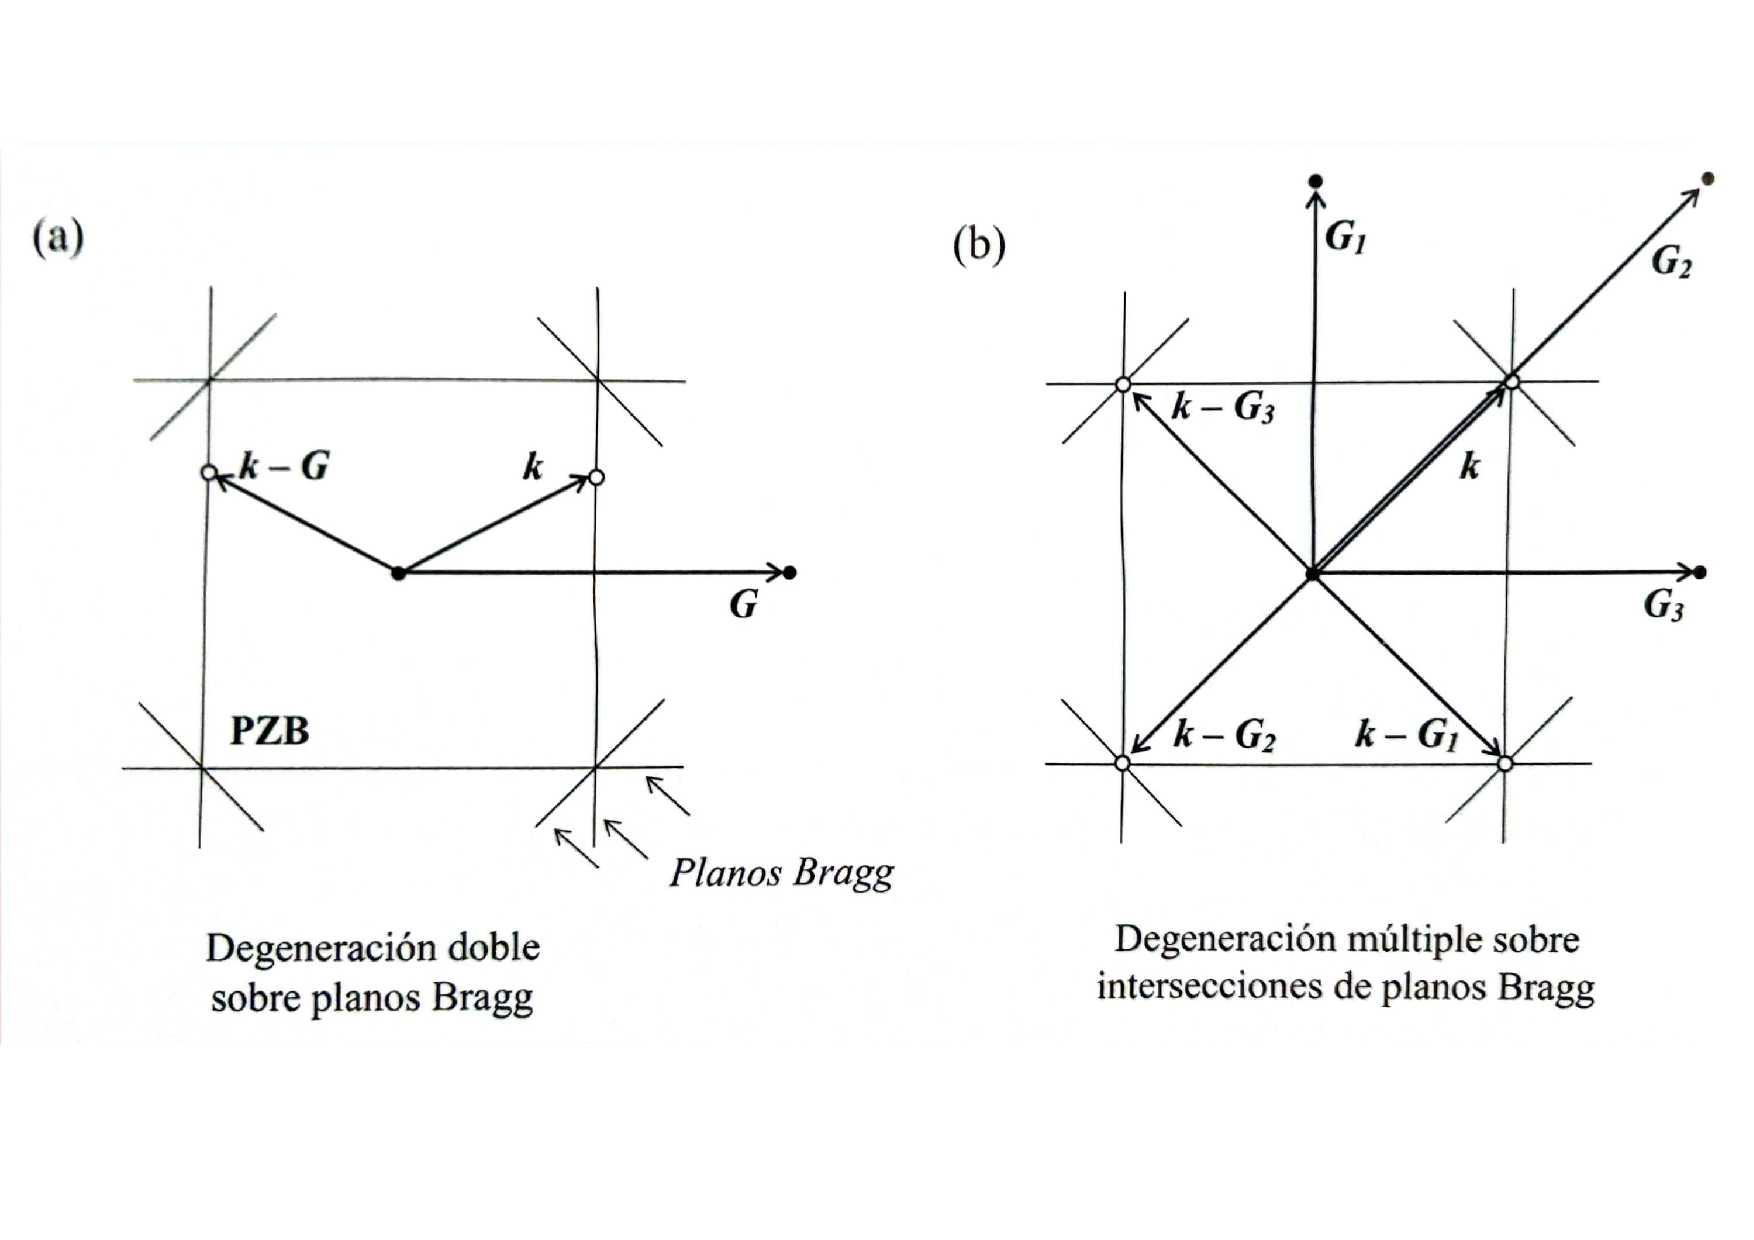
\includegraphics[scale=0.35]{Cuerpo/Ch_07/Fotos libro 2.pdf}
    \caption{(a) Ejemplo de estados doblemente degenerados sobre planos Bragg de una red cuadrada. (b) Estados cuádruplemente degenerados sobre las esquinas de la PZB de una red cuadrada.}
    \label{Fig:07-02}
\end{figure}    

Estas condiciones se cumplen para estados cerca de los planos de Bragg dado que verifican $|\kn|\approx |\kn-\Gn|$ (figura \ref{Fig:07-02} (a)), aunque no cerca de sus intersecciones donde la degeneración es mayor (figura \ref{Fig:07-02} (b)) . El sistema de ecuaciones (\ref{Ec:07-04-05}) resulta (se usa $U_\Gn=U_{-\Gn}$ por la simetría de inversión de $U$):

\begin{equation}
    \begin{split}
    \ccorchetes{\varepsilon-\varepsilon_0 (\kn - \Gn)} C_{\kn-\Gn} \ = & \ U_\Gn C_\kn \\
    \ccorchetes{\varepsilon-\varepsilon_0 (\kn)} C_\kn \ = & \ U_\Gn C_{\kn-\Gn}
    \end{split} \label{Ec:07-04-08}
\end{equation}
que en forma matricial queda como

\begin{equation}
\begin{pmatrix}
\varepsilon - \varepsilon_0 (\kn) & - U_\Gn \\
U_\Gn & \varepsilon - \varepsilon_0 (\kn - \Gn)
\end{pmatrix} \begin{pmatrix}
C_\kn \\
C_{\kn - \Gn}
\end{pmatrix} = 
\begin{pmatrix}
0 \\
0
\end{pmatrix}
\end{equation}

La solución se obtiene igualando a cero el determinante de la matriz, resultando

\begin{equation}
    \varepsilon = \frac{1}{2} \ccorchetes{\varepsilon_0 (\kn) + \varepsilon_0 (\kn - \Gn)} \pm \sqrt{\parentesis{\dfrac{\varepsilon_0 (\kn) + \varepsilon_0 (\kn - \Gn)}{2}}^2 + |U_\Gn|^2}
\end{equation}
En particular, exactamente sobre los planos de Bragg se tiene que

\begin{equation}
    \varepsilon = \varepsilon_0 (\kn) \pm |U_\Gn | \label{Ec:07-04-11}
\end{equation}
o sea, existe un \textit{intervalo prohibido de energía} de amplitud $2|U_\Gn|$. Es fácil comprobar que, además 

\begin{equation}
    \parciales{\varepsilon}{\kn} = \frac{\hbar^2}{m} \parentesis{\kn - \frac{\Gn}{2}}
\end{equation}
lo que implica que que las superficies de energía constante perpendiculares a los planos de Bragg, como se ilustra en la figura \ref{Fig:07-03}. La figura \ref{Fig:07-04} ilustra la aparición de las bandas prohibidas en las fronteras de zona para el ejemplo en 1D.

\begin{figure}[h!] \centering
    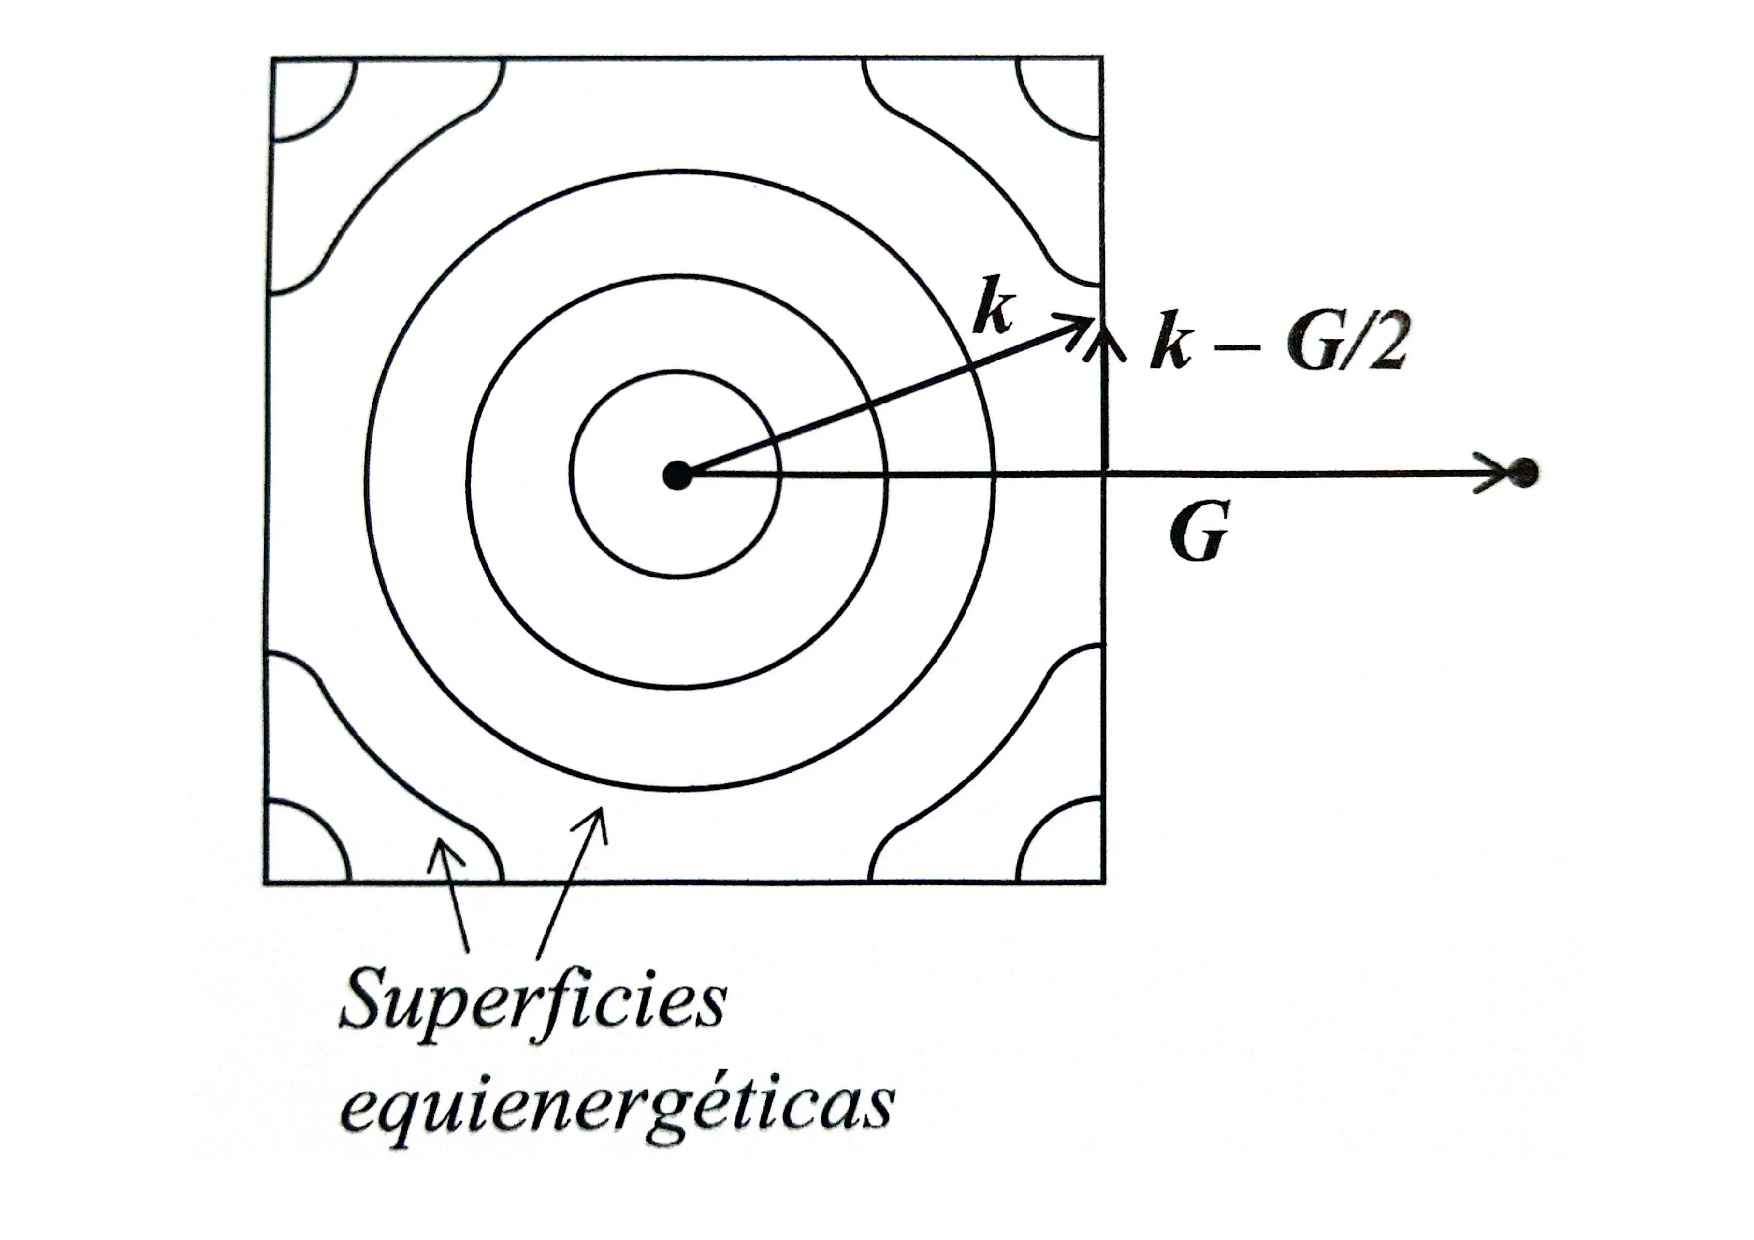
\includegraphics[scale=0.35]{Cuerpo/Ch_07/Fotos libro 3.pdf}
    \caption{Ejemplo de contornos equienergéticos en la PZB de una redcuadrada en la aproximación de electrones cuasilibres. Lejos de los planos de Bragg la aproximación de electrones libres es buena y los contornos son circulares. En los planos de Bragg, según se abre un gap de amplitud $2|U_{\Gn}|$. Según los contornos son perpendiculares a los planos de Bragg.}
    \label{Fig:07-03}
\end{figure}    

\begin{figure}[h!] \centering
    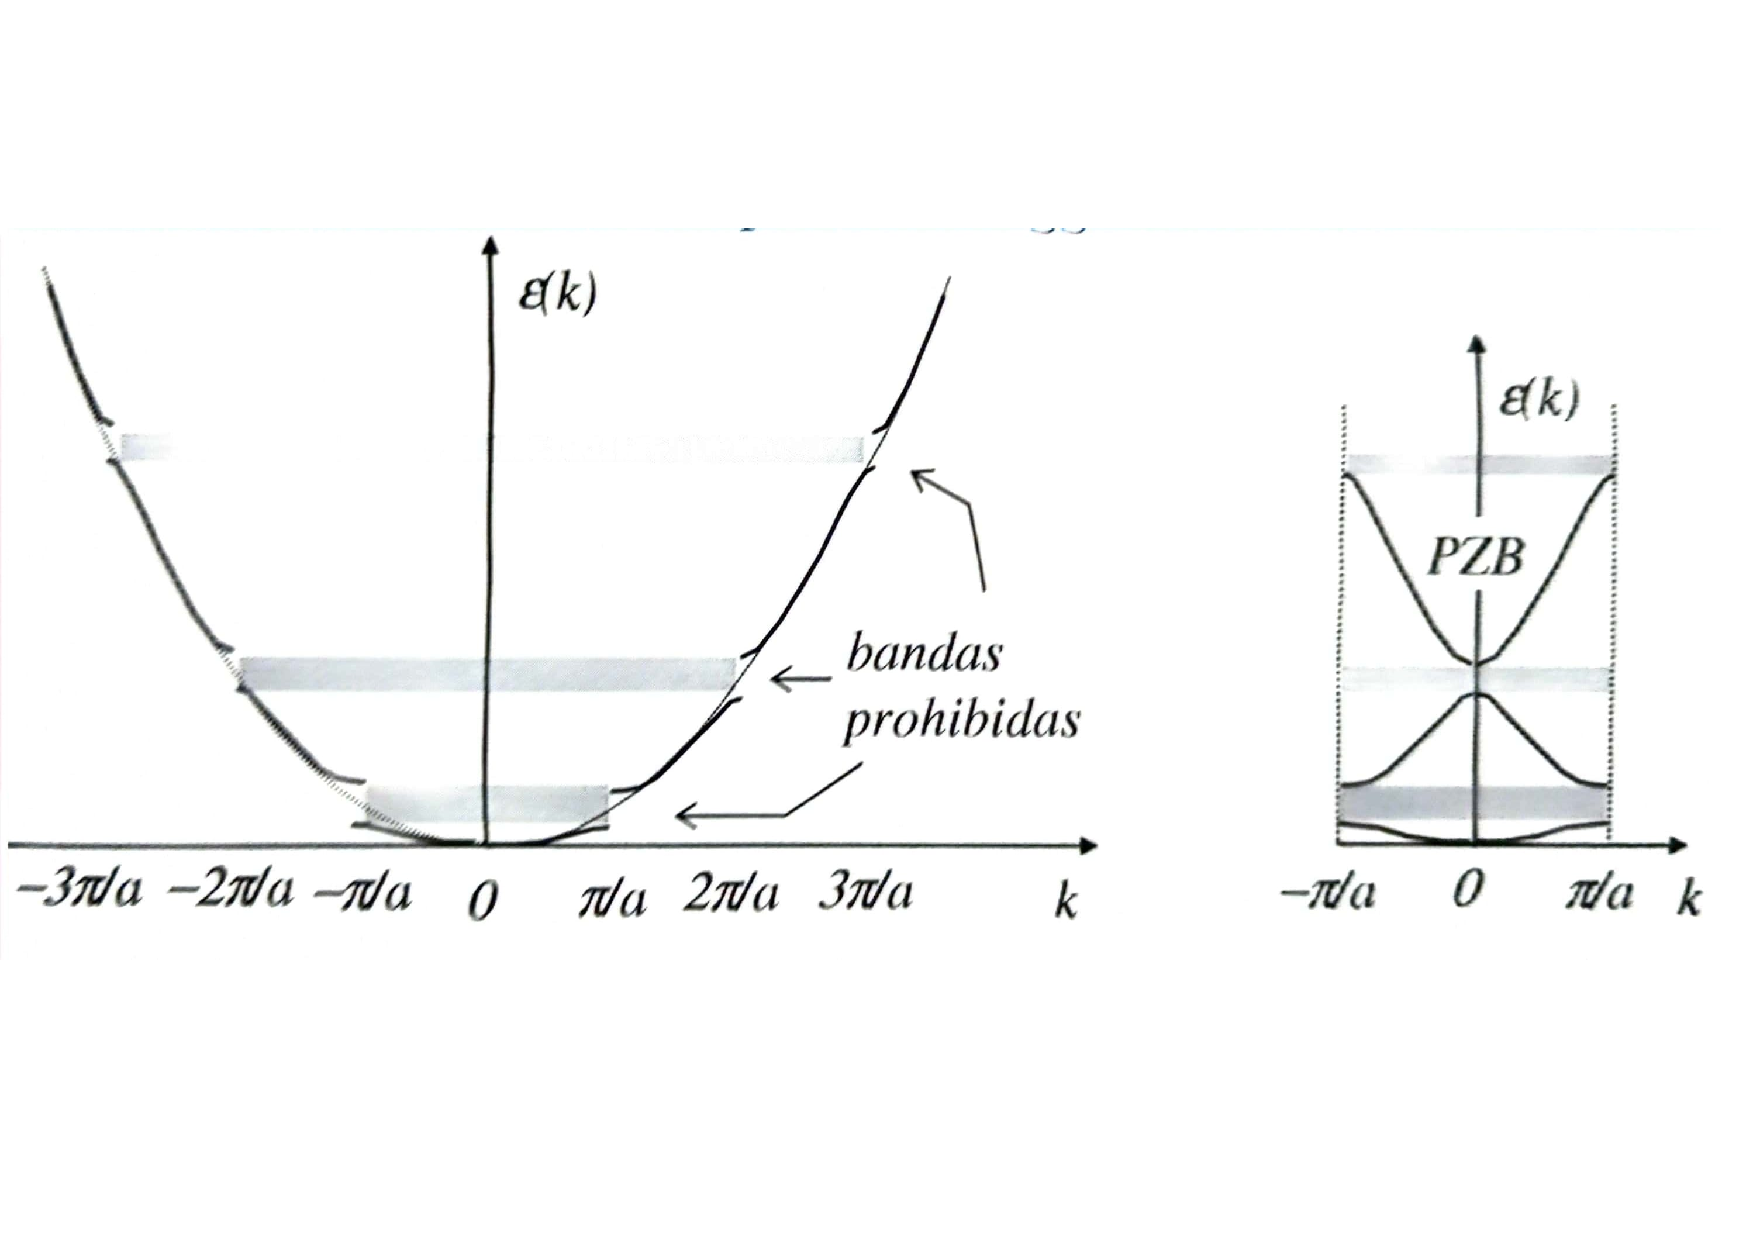
\includegraphics[scale=0.35]{Cuerpo/Ch_07/Fotos libro 4.pdf}
    \caption{Bandas prohibidas en los esquemas en zona extendida (izquierda) y reducida (derecha).}
    \label{Fig:07-04}
\end{figure}    

La existencia de intervalos prohibidos (o \textit{gaps}) de energía en las fronteras de zona es el resultado más importante de este Capítulo \ref{Ch:07}. Como sobre los planos de Bragg $\kn$, verifica la condición de difracción, la aparición de bandas prohibidas de energía peude asociarse a un fenómeno de difracción interna de la onda electrónica asociada. En efecto, al sustituir (\ref{Ec:07-04-11}) en (\ref{Ec:07-04-08}) se obtiene $C_\kn = \pm \text{sgn}(U_\Gn) C_{\kn-\Gn}$\footnote{el signo de $U_\Gn$}, lo que quiere decir que, por efecto del potencial, la onda plana $e^{i \kn \cdot \rn}$ , lleva asociada una nueva onda $e^{i(\kn -\Gn)\cdot \rn}$ con la que se combina (con el mismo peso) para dar la función de ondas final, que además tiene la forma de odna estacionaria. La presencia de $e^{i(\kn - \Gn)\cdot \rn}$ es coherente con la idea de una onda electrónica difractada. 

\section{Electrones fuertemente ligados}

Se trata de una aproximación al cálculo de las funciones de onda y energías electróncias en la que se parte de los estados atómicos yse estudia perturbativamente el efecto de otros átomos próximos. Es un efoque útil para describir los electrones de bandas internas $d$ de los metales de transición o los de los aislantes.

Consideramos para simplificar una cristal monoatómico, y denotamos por $\epsilon_n$, $\phi_n$ las energías y autoestados atómicos: $H_{\text{at}} \phi_n = \epsilon_n \phi_n$. La aproximación lineal es probar como solución

\begin{figure}[h!] \centering
    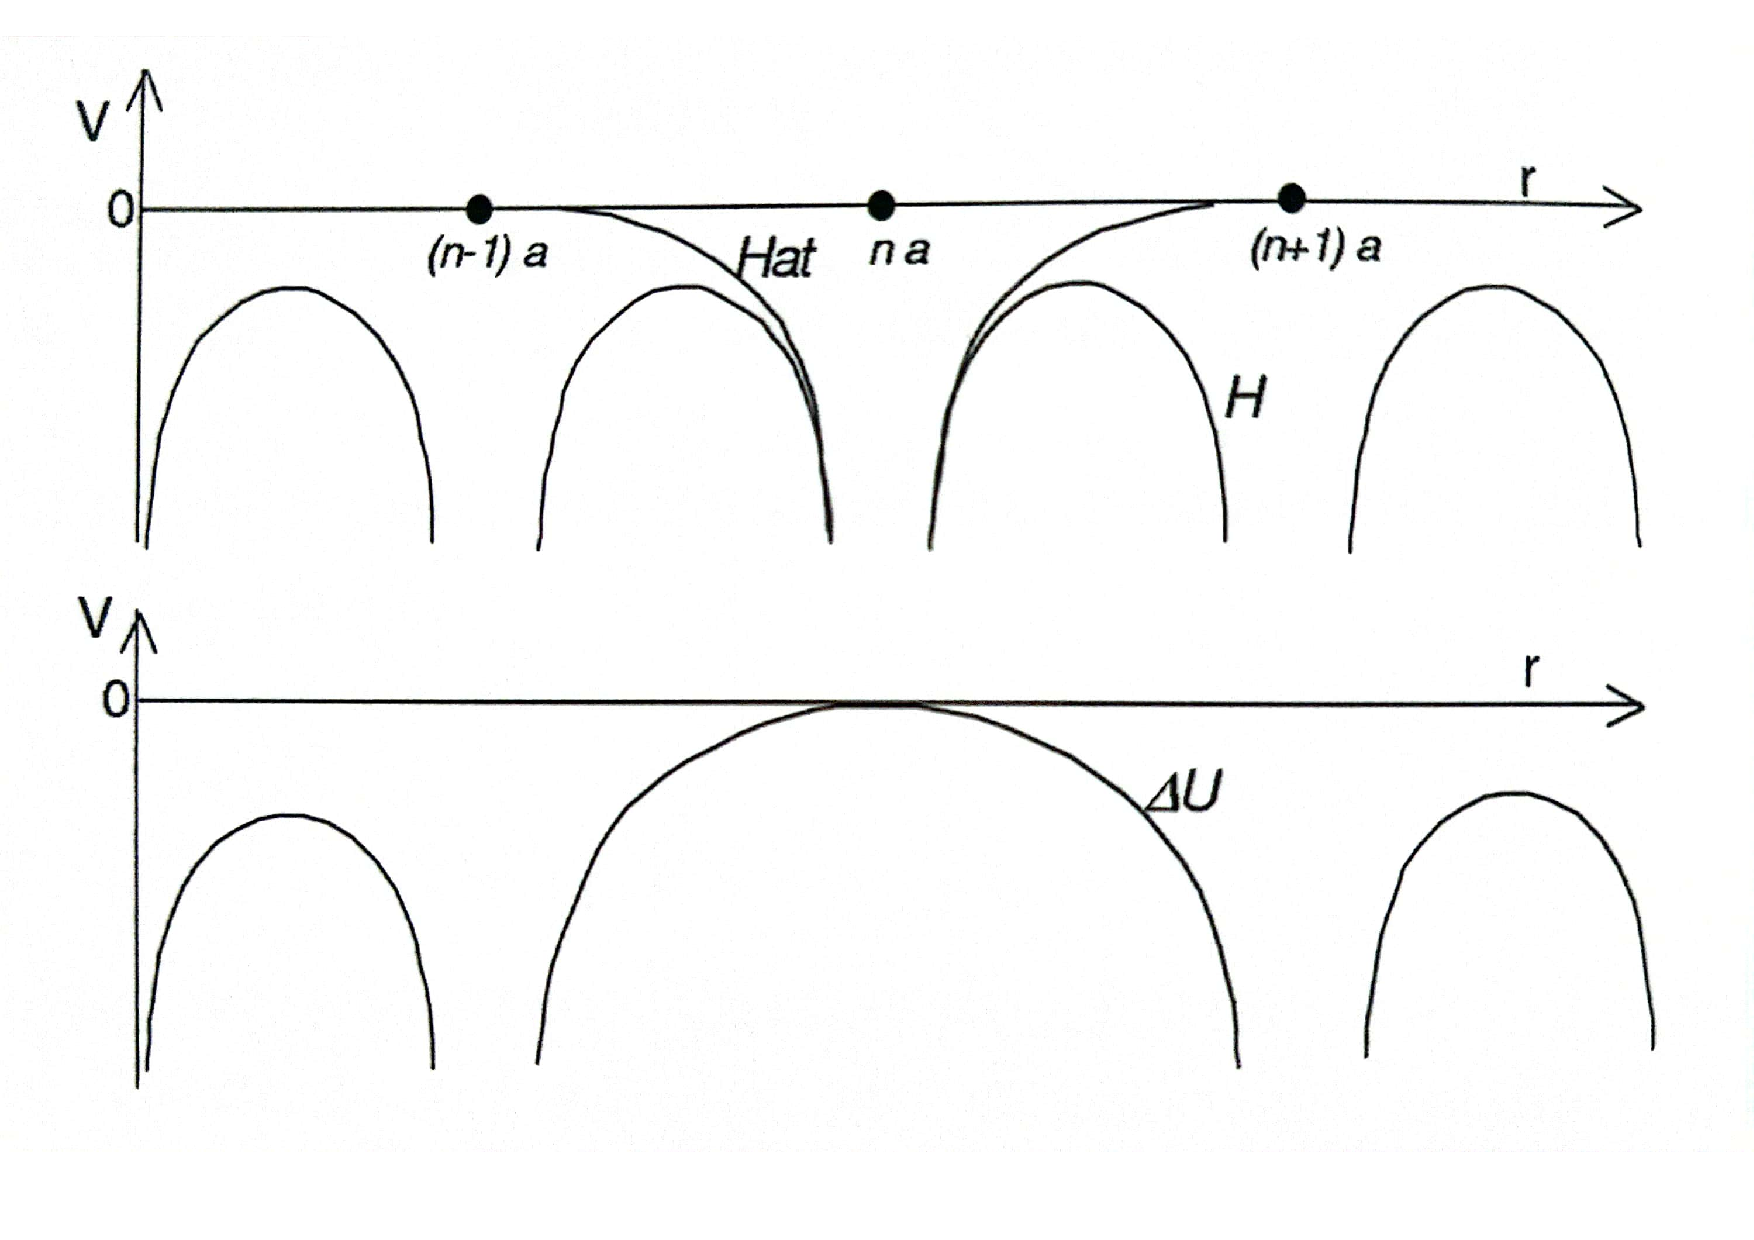
\includegraphics[scale=0.5]{Cuerpo/Ch_07/Fotos libro 5.pdf}
    \caption{Potencial periódico expresado como suma de un potencial atómico más una perturbación.}
    \label{Fig:07-05}
\end{figure}    
\begin{figure}[h!] \centering
    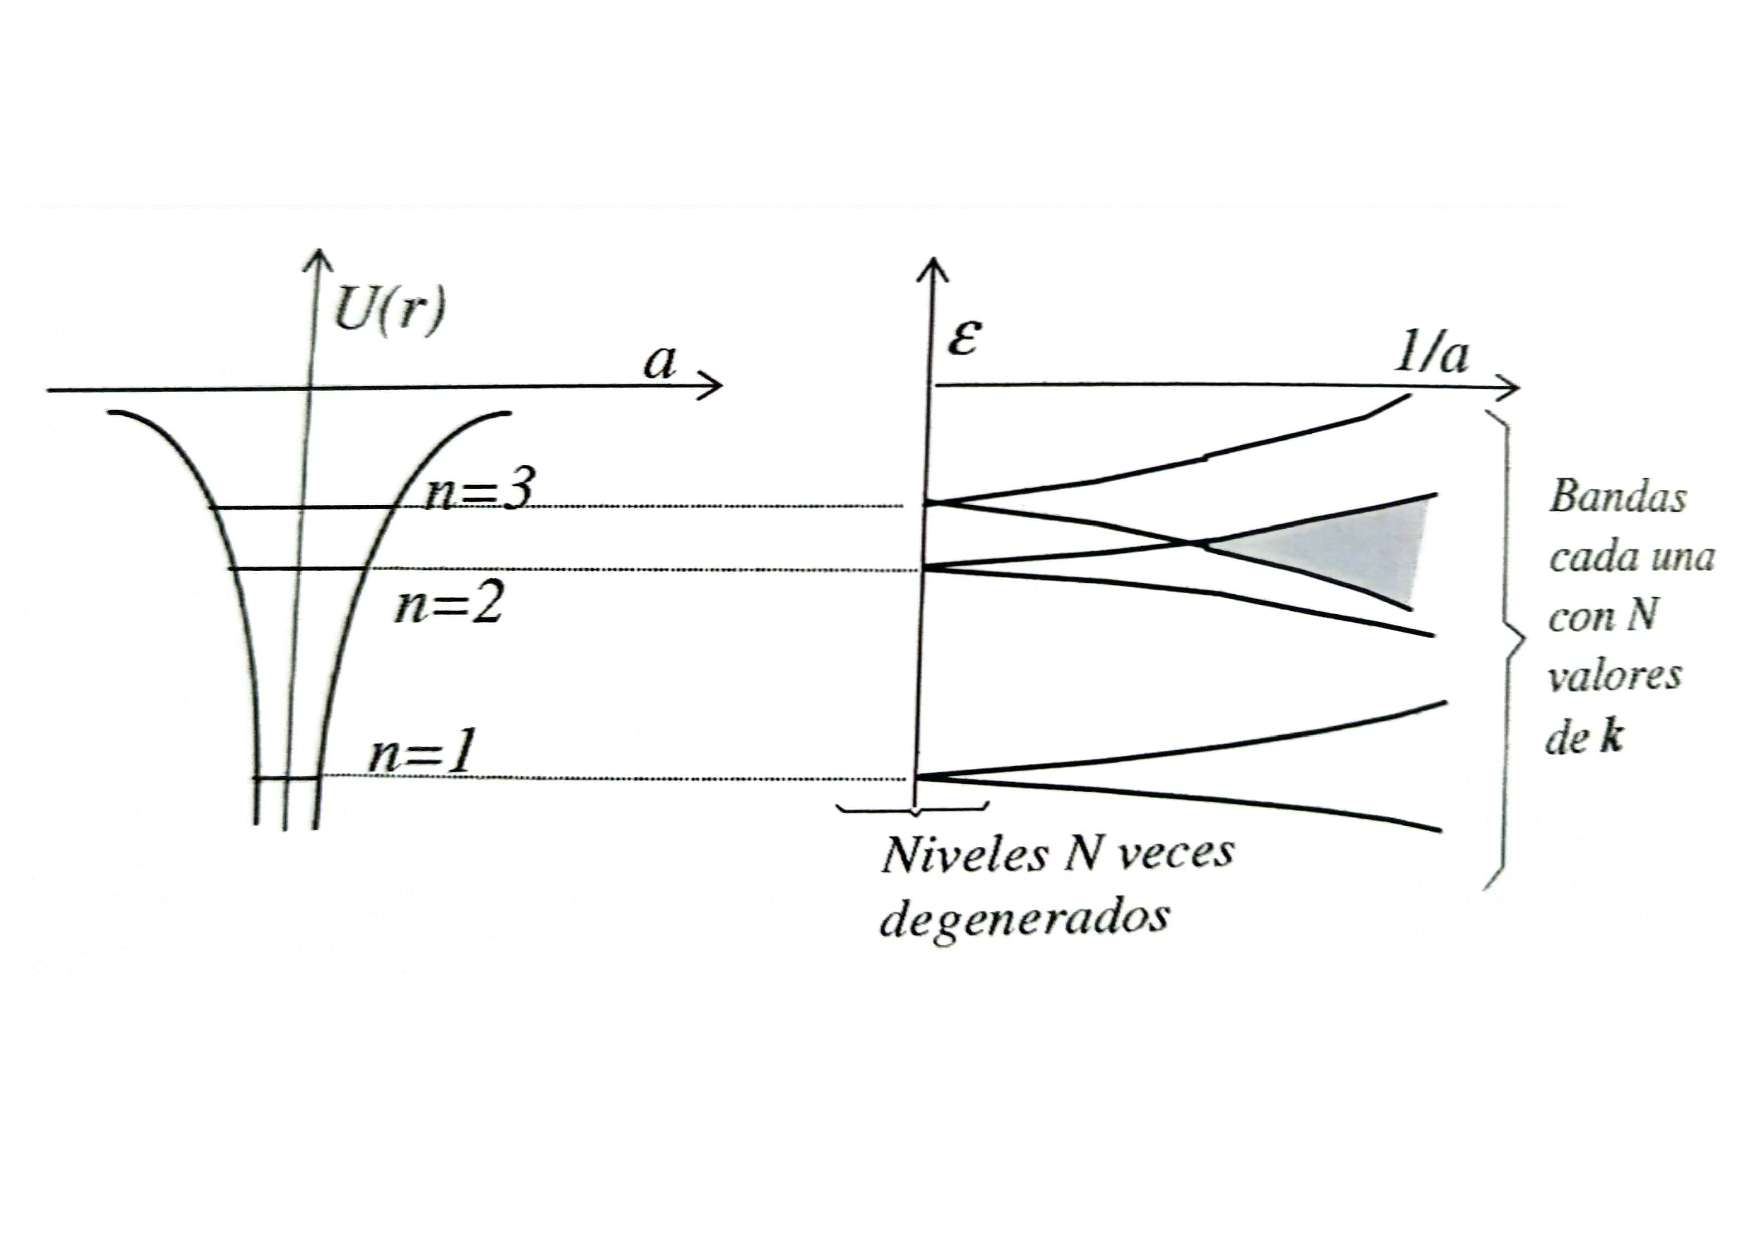
\includegraphics[scale=0.5]{Cuerpo/Ch_07/Fotos libro 6.pdf}
    \caption{Bandas de energía a partir de la aproximación de electrones fuertemente ligados. La zona sombreada representa el solapamiento entre la 1ª y 2ª bandas.}
    \label{Fig:07-06}
\end{figure}    

\section{Superficie de Fermi y zonas de Briollouin}
\begin{figure}[h!] \centering
    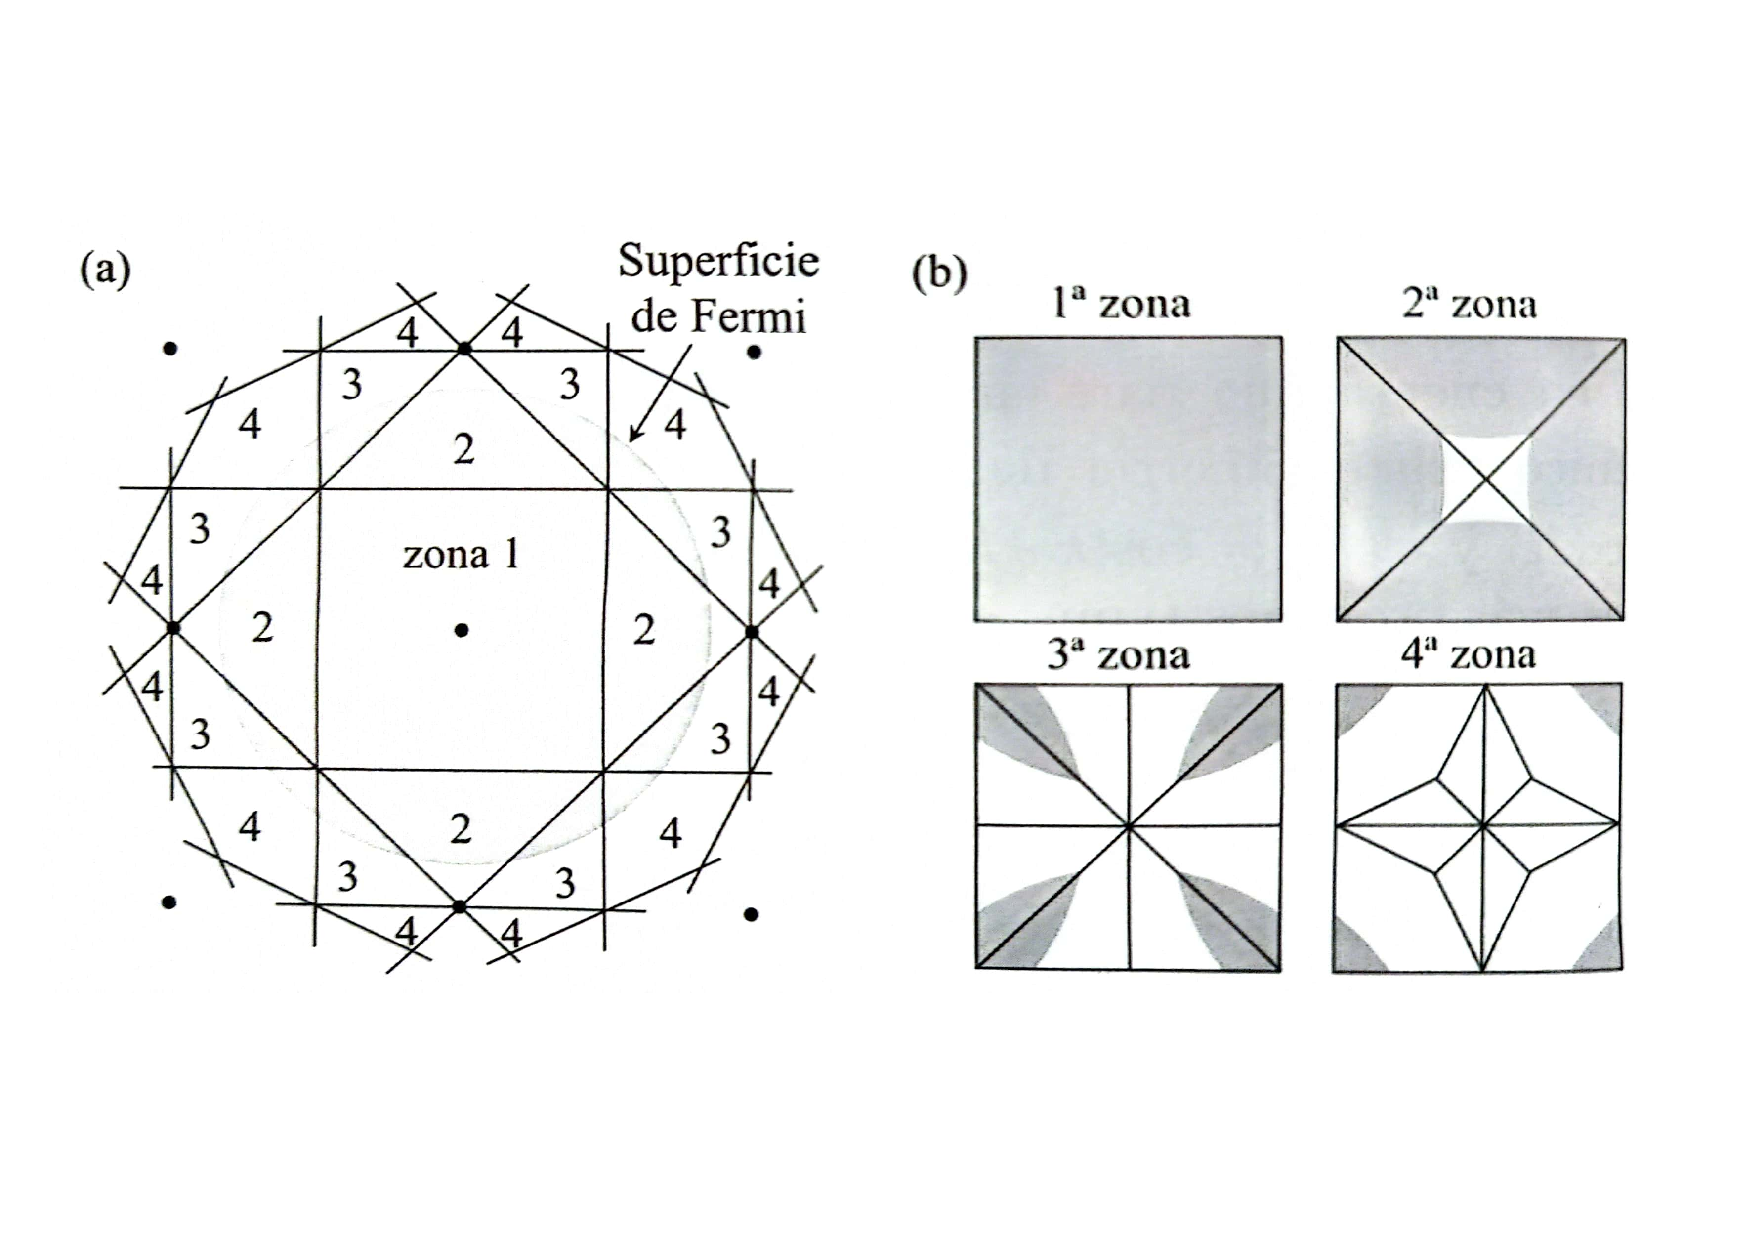
\includegraphics[scale=0.5]{Cuerpo/Ch_07/Fotos libro 7.pdf}
    \caption{1ª, 2ª, 3ª y 4ª zonas de Brillouin para una red cuadrada 2D, según los esquemas en zona extendida (a) y reducida (b). En gris se representan los estados ocupados.}
    \label{Fig:07-07}
\end{figure}    
\begin{figure}[h!] \centering
    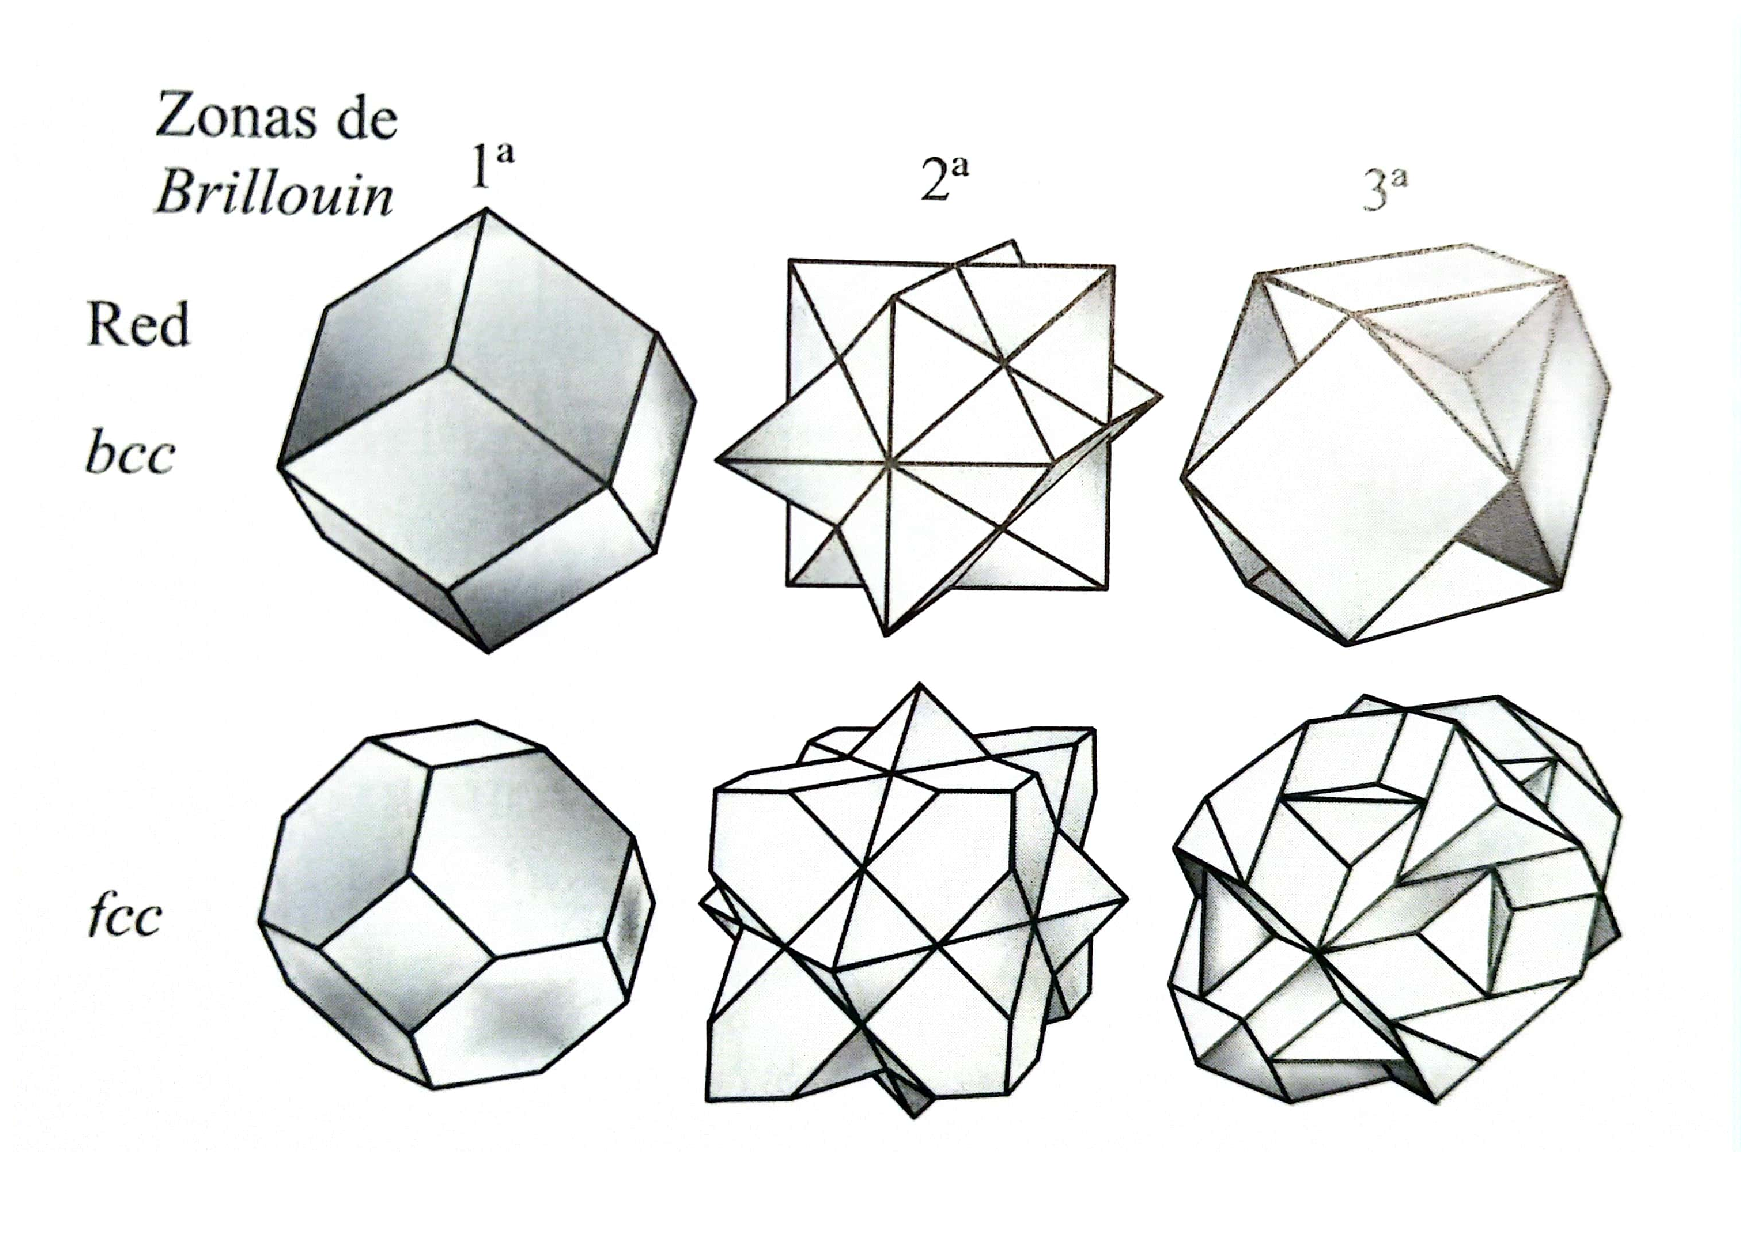
\includegraphics[scale=0.5]{Cuerpo/Ch_07/Fotos libro 8.pdf}
    \caption{Primeras zonas de Brillouin para las estructuras \bcc y \fcc, según el esquema en zona reducida.}
    \label{Fig:07-08}
\end{figure}    
\begin{figure}[h!] \centering
    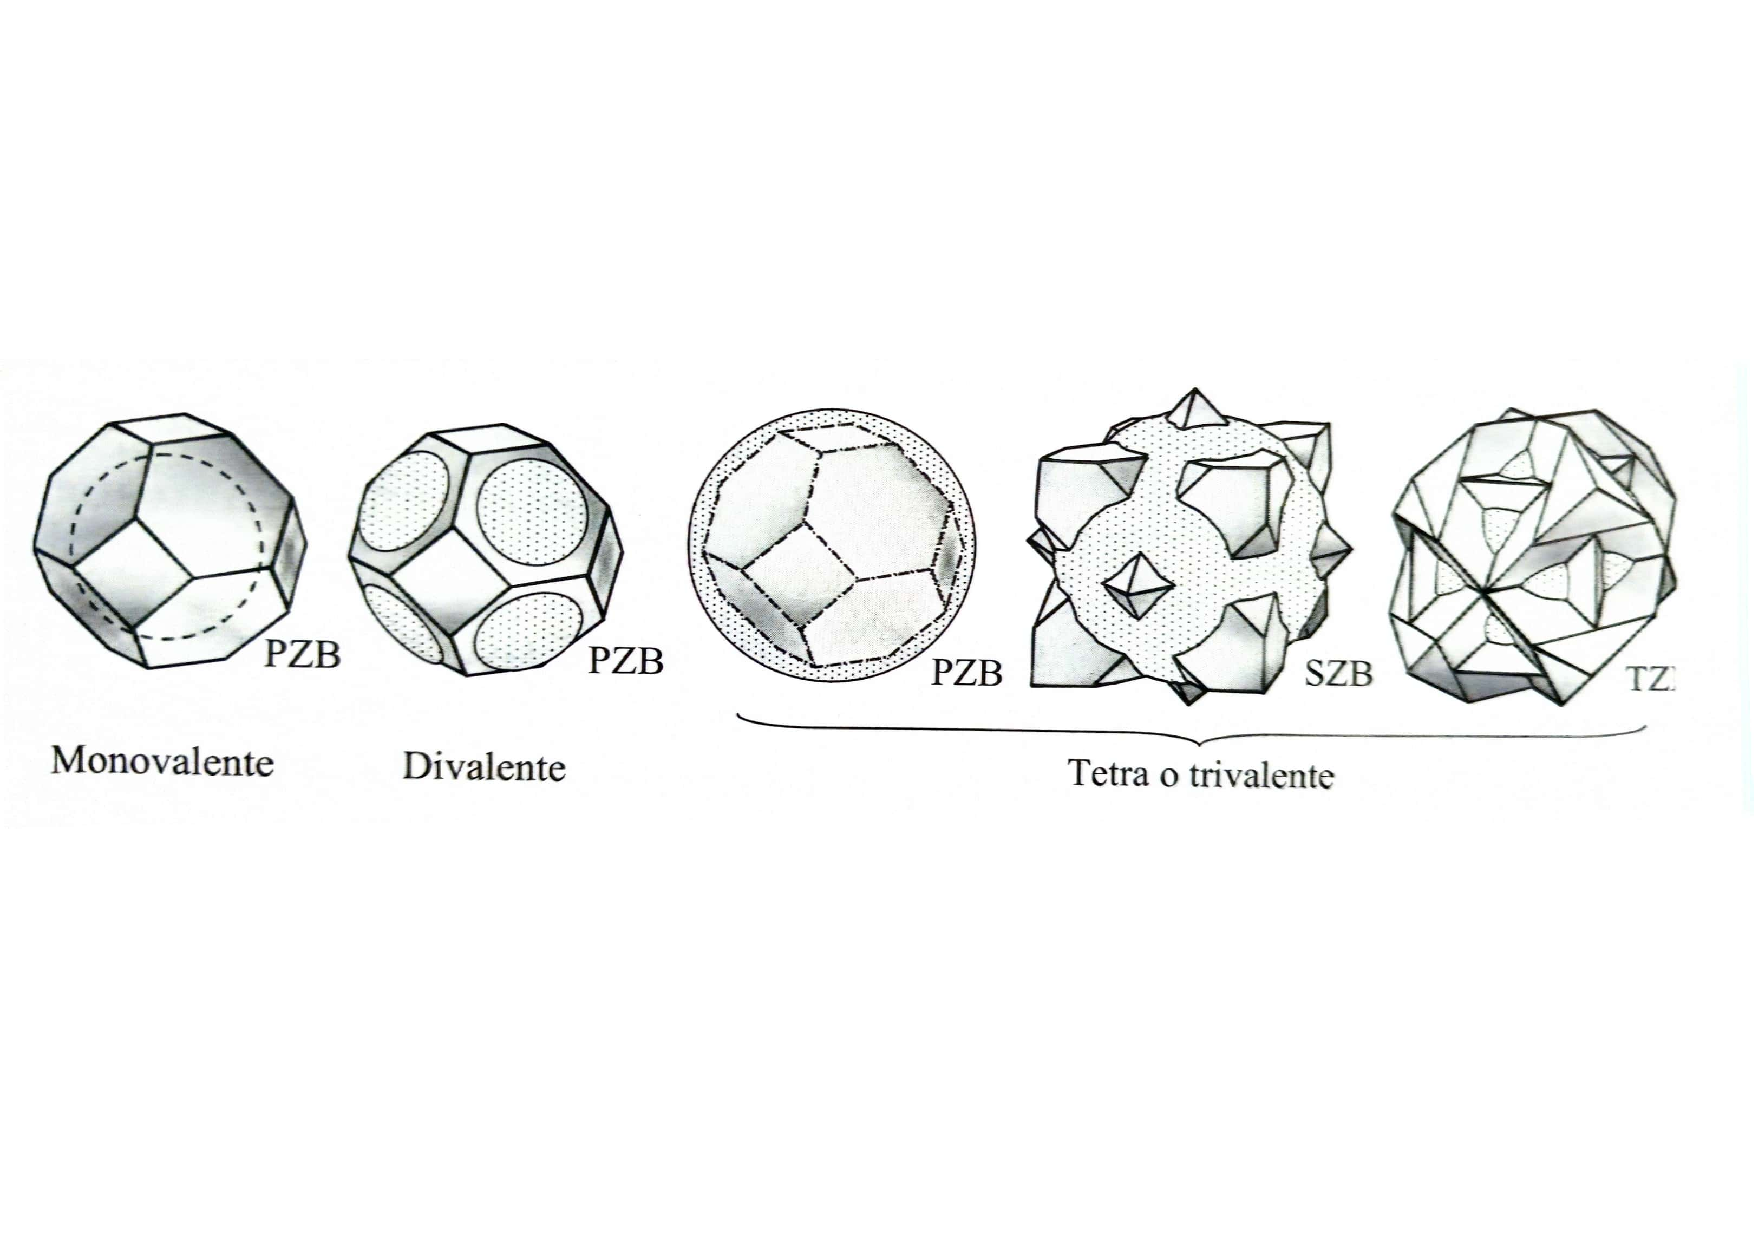
\includegraphics[scale=0.5]{Cuerpo/Ch_07/Fotos libro 9.pdf}
    \caption{Relación entre las primeras zonas de Brillouin de la estructura \fcc y la superficie de Fermi de electrones libres (esférica), según la valencia atómica.}
    \label{Fig:07-09}
\end{figure}    


\section{Metales, aislantes y semiconductores}
\begin{figure}[h!] \centering
    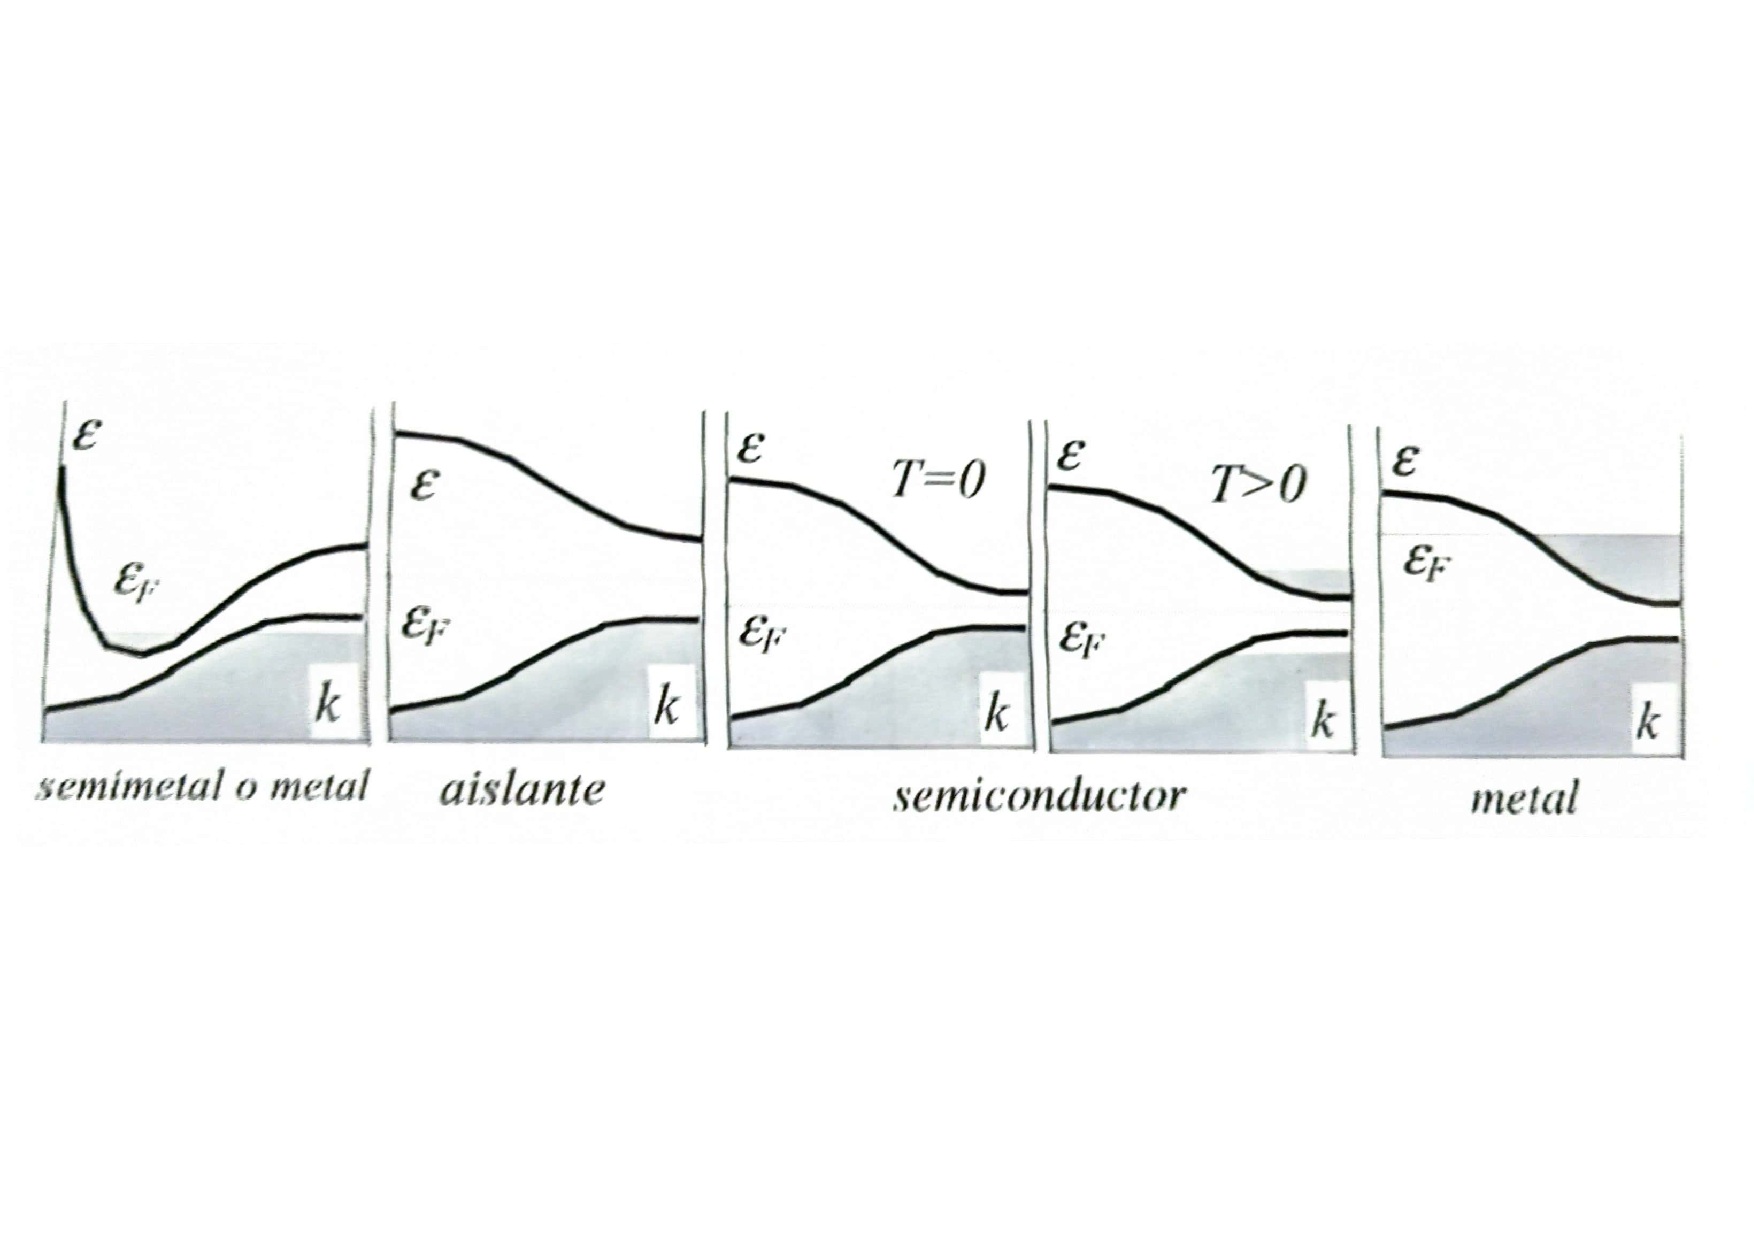
\includegraphics[scale=0.5]{Cuerpo/Ch_07/Fotos libro 10.pdf}
    \caption{Clasifiación de los sólidos según la relación que hay entre el nivel de Fermi y la estructura de bandas.}
    \label{Fig:07-10}
\end{figure}    
